 % !tex root= main.tex
  
\section{Formation de la Jonction Neuromusculaire}
\label{sec:IntroSynapse}
	La \gls{jnm} est une synapse qui permet la transmission nerveuse entre le motoneurone, un neurone dont le corps cellulaire est localisé dans la moëlle épinière, et la fibre musculaire squelettique. La \gls{jnm} est indispensable à la survie de l'organisme, permettant les mouvements volontaires et la respiration. De part sa grande taille et sa facilité d'accès, la \gls{jnm} est depuis longtemps le modèle préférentiel d'étude des synapses du point de vue structural, développemental, et physiologique. Chez les vertébrés, le neurotransmetteur présent à la \gls{jnm} est l'\gls{ach}. 

	L'apposition de l'élément pré-synaptique (axone) sur l'élément post-synaptique (fibre musculaire) requiert au préalable une différenciation post-synaptique qui se manifeste par la présence d'agrégats de \gls{achr} au milieu de la fibre musculaire. L'étape de formation d'agrégats aneuraux de \gls{achr} qui se déroule avant la reconnaissance du muscle par l'axone et l'ancrage de celui-ci sur l'élément post-synaptique se nomme "muscle pre-patterning" \cite{Wu2010a, Gordon2012}. Elle dépend entièrement de la présence de \gls{musk}, un récepteur tyrosine kinase qui va avoir plusieurs rôles dans la formation de la \gls{jnm} : attirer l'axone, stimuler la formation et le remodelage des agrégats de \gls{achr} chez l'embryon ainsi que maintenir la synapse chez l'adulte \cite{Hesser2006}.

	Lors du développement, le cône de croissance de l'axone se dirige vers l'élément post-synaptique (\cref{fig:FormaJNM}). Quand les deux éléments entrent en contacts (au jour embryonnaire E14 chez la souris), des cascades de signalisation sont initiées, ce qui résulte en la différentiation des parties pré- et post-synaptiques \cite{Sanes1999}, avec notamment une redistribution des clusters de \glspl{achr}, qui ne sont plus présent dans les régions extrasynaptiques, mais uniquement concentrés au niveau de la synapse.

	\begin{figure}[h]
		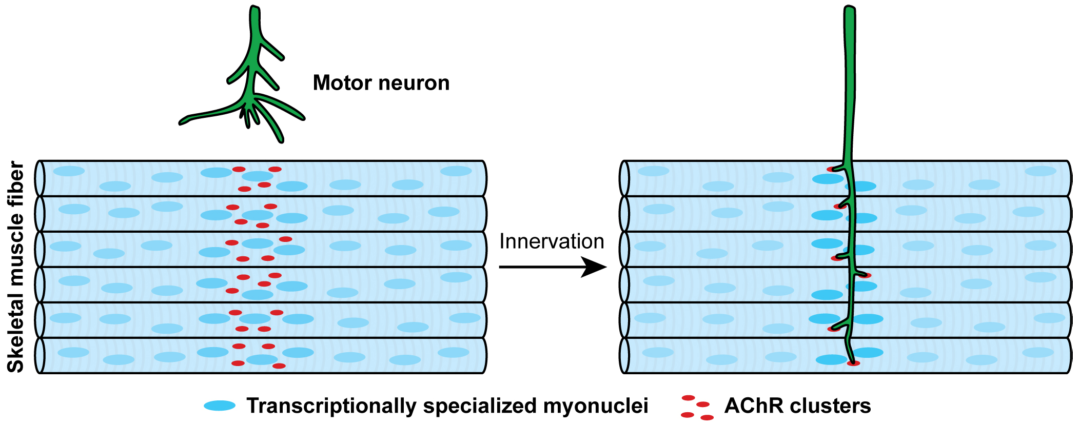
\includegraphics[width=\textwidth]{./Images/formation_jnm.png}
		\caption{Formation de la \gls{jnm}.} 
		\descfig{Figure issue de Burden \emph{et al.} 2018 \cite{Burden2018}.}
		\label{fig:FormaJNM}
	\end{figure}

	Ainsi, l'acteur majeur du développement de la synapse neuromusculaire est donc \gls{musk}, qui sert de plateforme de signalisation à la fois durant les étapes de pré-patterning, puis durant les étapes de mise en place et de maturation de la synapse.
		
\section{Le récépteur \acrshort{musk}, une molécule clef de la synaptogénèse}
\label{sec:IntroMuSK}	

	\begin{wrapfigure}{l}{0.25\textwidth}
		\centering{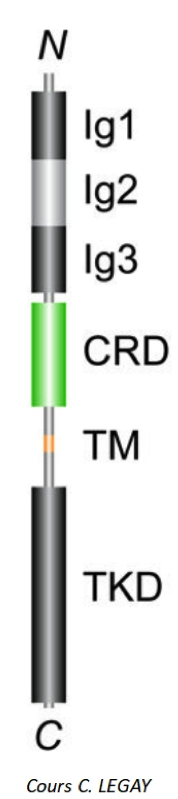
\includegraphics[width=0.1\textwidth]{./Images/MuSKReceptor.png}}
		\caption{Récepteur \gls{musk}}
		\descfig{Ig : Domaine immunoglobuline, CRD : \emph{Cysteine Rich Domain}, TM : Domaine transmembranaire,TKD : Domaine tyrosine kinase.}
		\label{fig:RMuSK}
	\end{wrapfigure}
	
	\acrfull{musk} est un récepteur découvert dans l'organe électrique de la raie \emph{Torpedo california} \cite{Jennings1993}. L'expression de ce récepteur à d'abord été quantifiée dans les cellules musculaires et localisée au niveau de la \gls{jnm}. \gls{musk} est un récepteur tyrosine-kinase de 98kDa, dans lequel on distingue trois parties : un ectodomaine (partie N-terminale), un domaine transmembranaire, et un domaine cytoplasmique qui porte l'activité kinasique (voir \cref{fig:RMuSK}). 
	
	La partie extracellulaire comporte trois domaines de type \gls{ig}, dont le domaine \gls{ig}1 a récemment été impliqué dans la liaison avec le \gls{lrp}4 \cite{Zhang2011}, ainsi qu'un domaine Frizzled-like, riche en cystéines (\gls{crd}) \cite{Jing2009}.
	
	\gls{musk} possède trois ligands connus : l'Agrine (via \acrshort{lrp}4), un collagène spécifique associé à l'\Gls{ache} appelé \acrshort{colq}, et les \Glspl{wnt}, tous nécessaire au développement complet de la synapse. Un défaut de signalisation de l'un d'entre eux entraîne ainsi des défauts structuraux et/ou fonctionnels de la synapse. L'Agrine joue un rôle prépondérant par rapport aux autres ligands.
	
	%Précédemment à la fin de section 1.
	L'Agrine est le ligand historique de \gls{musk} \cite{Glass1996}, dont une isoforme neuronale est sécrétée par l'axone au contact de la cellule musculaire. Plus récemment, des travaux ont montré que l'Agrine se fixait en fait sur le co-récépteur de \gls{musk} : \gls{lrp}4 \cite{Zhang2008,Kim2008}. Suite à l'activation par l'Agrine de \acrshort{lrp}4, deux complexes \gls{musk}/\gls{lrp}4 vont s'assembler, et cet assemblage tétramérique permettrait une phosphorylation optimale de \gls{musk}, et donc une différenciation de la synapse et de l'agrégation des \gls{achr} \cite{Zong2012}.
	
	La présence de \gls{musk} dans le cerveau a longtemps été ignorée, du fait de sa faible expression dans cette organe, quantifiée dans le passé par Northern Blot, une méthode de détection des \acrshort{arnm} peu sensible. Cependant, de nouvelles techniques, telle que l'\gls{his} ou bien la \gls{qpcr}, ont permis de montrer que le récepteur était bien présent dans le tissu cérébral, principalement au niveau des neurones du cortex, du cervelet, et de l'hippocampe \cite{Garcia-Osta2006, Ksiazek2007}. Le récepteur \gls{musk} semble aussi être exprimé fortement dans les astrocytes \cite{Sun2016}, à des taux jusqu'à 5 fois supérieur à son expression dans les muscles squelettiques.
	
	Bien que sa présence soit prouvée dans le cerveau, le rôle de \gls{musk} dans cette structure reste assez méconnu. 
	
	%WTF a voir ou inserer.
	% où avec son co-récepteur \gls{lrp}4 il régulerait la transmission glutamatergique par l'intermédiaire de la libération d'ATP et une signalisation liée à l'agrine.
	
	\todo{a améliorer}
	Au niveau du \gls{snc}, deux isoformes de \gls{musk} semblent être exprimées \cite{Garcia-Osta2006}. La première isoforme, de 2644pbs, est identique à une isoforme générée par épissage alternatif dans le muscle \cite{Valenzuela1995}, sans qu'aucun rôle ne lui soit connu pour l'instant. La seconde isoforme est plus courte : 2359pbs, et présente une délétion du troisième domaine \gls{ig}. Les deux isoformes présentent une alanine à la position 454 qui remplace une délétion de 8 acides aminé de l'ectodomaine. Une autre isoforme ayant le domaine \gls{ig}3 supprimé serait impliquée dans l'agrégation des \gls{achr} \cite{Hesser1999}.
	
	Grâce à des techniques de knockdown du gène par séquence antisens au niveau de l'hippocampe, il apparaîtrait que la présence de \gls{musk} dans le cerveau serait nécessaire mais non indispensable à la formation de la mémoire à moyen et long-terme \cite{Garcia-Osta2006}. La voie \gls{creb} est une voie impliquée dans la formation de la mémoire au niveau de l'hippocampe \cite{Silva1998, Kandel2012,Kida2014,Ortega-Martinez2015}, qui serait médié par la phosphorylation de \gls{creb} suite a la libération de \acrshort{camp} \todo{par quoi ?}, augmentant son activité transcriptionnelle. Un modèle propose que l'activation de \gls{musk} activerait la cascade de signalisation de \gls{creb}, permettant la consolidation de la mémoire \cite{Garcia-Osta2006} . Ce modèle expliquerait également l'auto-régulation de \gls{musk} \cite{Moore2001}, dont le gène possède dans sa séquence promotrice un élément CRE-like liant \gls{creb} \cite{Kim2005}. De plus, \gls{musk} est nécessaire à la formation de la \gls{ltp} de l'hippocampe \cite{Garcia-Osta2006}.

\section{Les protéines \Acrshortpl{wnt}, ligands de \acrshort{musk}}
\label{sec:IntroWnt}	
	\begin{wrapfigure}{l}{0.4\textwidth}
		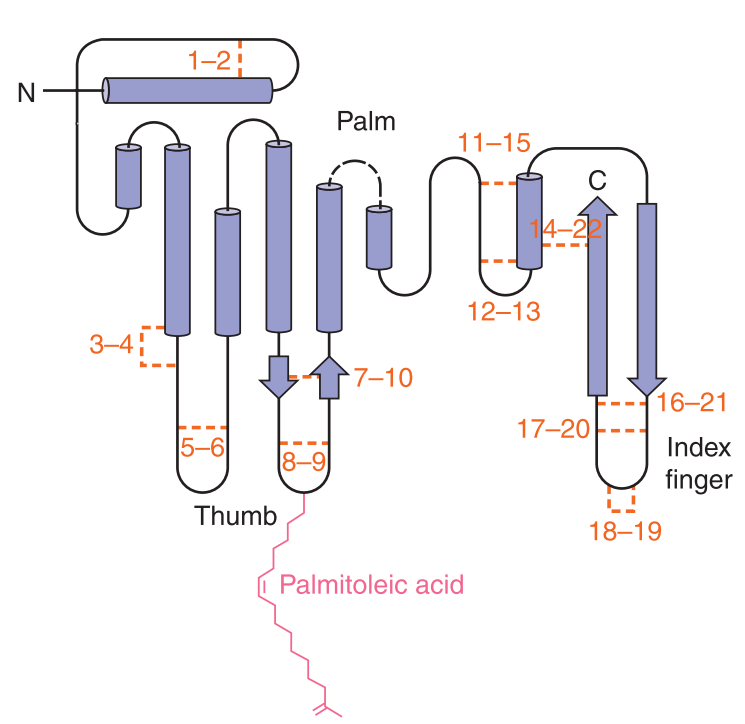
\includegraphics[width=0.4\textwidth]{./Images/WntProtein.png}	
		\caption{Structure d'une protéine \Gls{wnt} classique.}
		\descfig{Figure issue de Willert \& Nusse 2012 \cite{Willert2012}. En orange sont représentés les 22 résidus cystéines.}
		\label{fig:WntProt}
	\end{wrapfigure}
	
	%Les protéines \glspl{wnt} sont des ligands de \gls{musk}. Outre leur rôle dans la mise en place de la \gls{jnm} médiée par \gls{musk} \cite{Hall2000}, ces protéines sont connues pour leurs rôles prépondérant lors de la neurogénèse et de la mise en place de la connectivité dans les différentes structures du cerveau.
	
	Un des 3 ligands de \gls{musk}, les \Glspl{wnt}, ont un rôle avéré dans la formation de la \gls{jnm} \cite{Hall2000}, mais sont également connues pour leur fonction synaptogénique dans le cerveau.
	
	Les \Acrfullpl{wnt} sont des glycoprotéines sécrétées, de 40kDa pour 350 acides aminés, impliquées dans de nombreux processus développementaux tel que l'embryogenèse, la prolifération, la différenciation, la migration cellulaire, ou encore l'apoptose \cite{Miller2002, Willert2012}. 
	%En plus de leurs rôles durant le développement, les \Glspl{wnt} jouent également un rôle à l'age adulte dans la maintenance des tissus adultes. 
	
	La structure des \Glspl{wnt} est complexe, avec  de nombreux ponts disulfures caractéristiques de cette famille de protéines et d'hélices \textalpha{}. Deux modifications post-traductionelles sont courantes : la présence d'un acide palmitoléïque en Ser209 participant à la liaison avec leur récepteur \gls{fz} (voir \cref{fig:WntProt}), et la présence d'un acide palmitique en position Cys77 conservé au cours de l'évolution\cite{Takada2006}. Ces acides gras rendent les protéines \Gls{wnt} très hydrophobes, ce qui a retardé leurs caractérisations.
	
	On connaît actuellement 19 membres de cette famille de protéine chez la souris et chez l'humain. Classiquement, les \Glspl{wnt} se lient sur le domaine \gls{crd} de leur récepteur canonique \gls{fz}, associé aux co-récepteurs \gls{lrp}5 ou 6, mais il existe d'autres récepteurs non canoniques tels que : \gls{ror} \cite{Cadigan2006, Gordon2006, Green2008}, \gls{ryk} \cite{Bovolenta2006, Fradkin2010}, ou bien encore \gls{musk} \cite{Jing2009}, qui possèdent également un \gls{crd}.
	
	Les protéines \glspl{wnt} vont agir aux travers de différentes voies de signalisation dans la cellule : la voie canonique/\textbeta{}-catenin, la voie \gls{pcp}, et d'autres voies indépendantes de la voie \textbeta{}-catenin. La voie canonique fait intervenir \gls{gsk3}, qui participe à la dégradation de la \textBeta{}-catenin et à l'inactivation de la signalisation. 
	
	\emph{In vitro}, il a été montré que plusieurs \Glspl{wnt} interagissaient avec \gls{musk} : \Gls{wnt}2, 3a, 4, 6, 7b, 9a, et 11, qui ont des effets inhibiteurs, stimulateurs, ou sont neutres, sur l'aggragation des \gls{achr} \cite{Strochlic2012, Zhang2012, Barik2014}. Seules \gls{wnt}4, 9a et 11 vont conduire à une dimérisation de \gls{musk} et à son activation (\emph{in vitro}). Ceci est cohérent avec le fait que chez le Poisson-zèbre, l'orthologue de \gls{musk}, \emph{unplugged}, possède aussi un \gls{crd} qui interagit avec des protéines \Glspl{wnt} pour induire l'agrégation de \glspl{achr} \cite{Jing2009, Gordon2012}. \Gls{lrp}4 semble être également nécessaire à l'agrégation des \gls{achr} médié par les \gls{wnt}s \cite{Zhang2012}. De plus, une protéine centrale dans les différentes voie de signalisation des \Glspl{wnt}, \emph{Dishevelled}, a été montré comme pouvant interagir avec \gls{musk} \cite{Luo2002a}.

\section{\acrshort{musk} et \Acrshortpl {wnt} : Contexte de l'étude et but du stage}
\label{sec:Contexte}	
	Dans le but d'étudier le rôle de l'interaction des protéines \Glspl{wnt} et du domaine \gls{crd} de \gls{musk}, l'équipe de C. LEGAY à crée une souris transgénique dont le \gls{crd} était supprimé (\mcrd) \cite{Messeant2015, Messeant2017}. Il a ainsi été montré que le \gls{crd} était nécessaire à la \gls{jnm} à la fois pour sa formation et pour son maintien à l'age adulte, et que les \Glspl{wnt} 4 et 11 participaient activement à la mise en place de la synapse. De plus, un traitement au \gls{licl} (inhibiteur de la \gls{gsk3}) permet une réstauration du phénotype sauvage de la \gls{jnm} \cite{Messeant2015}. Cet effet du \gls{licl} indique que la voie \textbeta{}-catenin est impliqué dans la signalisation \Glspl{wnt}-\gls{musk}. %La voie \gls{pcp} serait également impliqué.
	
	Outre les symptômes de myasthénie congénitale lies à la mutation, les souris \mcrd présentaient des défauts centraux : durant son stage, une étudiante, Bertille Somon, a montré que les mutants mâles avaient des blessures importantes au niveau du dos, blessures qui n'étaient pas dues à des comportements d'agressivité entre souris. De plus, une analyse comportementale a été réalisée en collaboration avec le groupe du Dr Lanfumey (Centre de Psychiatrie et Neurosciences, Paris), et le \gls{nor} a révélé que les souris mutantes souffrent d'un déficit de la mémoire intermédiaire.
	
	\todo{Wnt MEMOIRE !!!!}
	Comme il a été montré que \gls{musk} est exprimé dans le cerveau adulte, principalement au niveau de l'hippocampe \cite{Garcia-Osta2006}, et que cette structure joue un rôle prépondérant dans la formation de la mémoire intermédiaire, l'objectif de mon stage était d'explorer le rôle de l'interaction de \gls{musk} et des \Glspl{wnt} dans le cerveau, utilisant pour cela les souris \mcrd. Dans cette perspective, je devais au préalable répondre à plusieurs questions : Est-ce que la structure du cerveau est affectée chez le mutant, quelles sont les cellules exprimant \gls{musk}, et quel est le niveau d'expression de \gls{musk} et \mcrd dans le cerveau ? Par ailleurs, j'ai également cherché à comprendre l'origine des défauts de comportement chez le mâle mutant.
	
	%\todo{wnt mémoire ???}